\section{问题二的模型建立与求解}

\subsection{总体思路}

问题二在每天 0:00 一次性确定当天 144 个时段的计划购电量与储能策略，负荷与光伏尚未揭晓时的缺口按 5 倍电价紧急购电。本文按``周期加权预测—整日联合残差场景—季节终端软区间混合整数规划—实际回放结算''的链条求解：所有预测和场景均只用历史信息，日末储电量传递至次日。正式期为 2025 年 2 月 1 日至 12 月 31 日，1 月仅用于构造历史残差和风险窗口。

\subsection{信息边界}

设 $d$ 为计划日期，在 $d$ 日 0:00 可用的信息集为

\begin{equation}
  \mathcal{I}_d = \{\, L_r(t),\ P_r(t) \mid r < d,\ t = 1,2,\dots,144 \,\},
  \label{eq:infoset}
\end{equation}

式中：$L_r(t)$ 与 $P_r(t)$ 分别为历史日期 $r$、时段 $t$ 的实际负荷电量与实际光伏电量；$\mathcal{I}_d$ 只包含 $d$ 日之前已经发生的数据。所有预测、残差归档、场景抽样与终端基准的风险微调均严格限制在 $\mathcal{I}_d$ 之内，当天实际值仅用于计划制定之后的紧急购电结算，以避免未来信息泄漏人为降低回测费用。

\subsection{24 小时周期加权平均预测模型}

附件 2 的实测数据表明，小区负荷具有明显的星期周期，而光伏发电由日内太阳辐照周期主导。据此，本文对负荷采用周周期加权平均、对光伏采用日周期加权平均，并用指数衰减系数对不同历史周期赋权\cite{ref4}。

\subsubsection{负荷预测}

对计划日 $d$ 的时段 $t$，取最近至多 4 个同星期历史时段的指数加权平均：

\begin{equation}
  \widehat{L}_d(t) = \frac{\displaystyle\sum_{k=1}^{K^L_d} \rho^{\,k-1} L_{d-7k}(t)}{\displaystyle\sum_{k=1}^{K^L_d} \rho^{\,k-1}},
  \qquad
  K^L_d = \min\left\{4,\ \left\lfloor \frac{d-1}{7} \right\rfloor \right\}.
  \label{eq:loadpred}
\end{equation}

式中：$\widehat{L}_d(t)$ 为计划日 $d$、时段 $t$ 的负荷电量预测值（kWh）；$L_{d-7k}(t)$ 为前第 $k$ 个同星期同期的实际负荷电量；$\rho$ 为衰减系数，取 0.8；$K^L_d$ 为可用历史周期数。当历史数据达到四周时，式~\eqref{eq:loadpred} 简化为 $L_{d-7},L_{d-14},L_{d-21},L_{d-28}$ 的加权平均，权重依次为 $1,0.8,0.8^2,0.8^3$。每个时段独立计算，不施加相邻时段平滑、样条或误差修正等额外处理。

\subsubsection{光伏预测}

对计划日 $d$ 的时段 $t$，取最近至多 7 个历史日同一时段的指数加权平均：

\begin{equation}
  \widehat{P}_d(t) = \frac{\displaystyle\sum_{k=1}^{K^P_d} \rho^{\,k-1} P_{d-k}(t)}{\displaystyle\sum_{k=1}^{K^P_d} \rho^{\,k-1}},
  \qquad
  K^P_d = \min\{7,\ d-1\}.
  \label{eq:pvpred}
\end{equation}

式中：$\widehat{P}_d(t)$ 为光伏电量预测值（kWh）；$P_{d-k}(t)$ 为前第 $k$ 日的实际光伏电量；$K^P_d$ 为可用历史天数，至多 7 天。考虑光伏出力的非负性，对预测值作非负保护 $\widehat{P}_d(t) \leftarrow \max\{\widehat{P}_d(t), 0\}$。

\subsection{24 小时联合残差场景生成}

点预测无法反映预测误差的分布特征。为在优化中刻画不确定性，本文按整日联合抽样构造场景\cite{ref3}。对历史预测日 $r$，待实际值全部揭晓后归档当日 0:00 实际发出的样本外残差：

\begin{equation}
  e^L_r(t) = L_r(t) - \widehat{L}_r(t), \qquad e^P_r(t) = P_r(t) - \widehat{P}_r(t),
  \label{eq:residual}
\end{equation}

式中：$e^L_r(t)$ 与 $e^P_r(t)$ 分别为历史日期 $r$、时段 $t$ 的负荷与光伏预测残差（kWh）。二者必须来自同一预测日，并以完整的 144 时段日块联合保存，以保留负荷误差与光伏误差之间以及日内各时段误差之间的相关性。

在 $d$ 日 0:00，只使用 $r<d$ 且已完成结算的残差块，历史日期 $r$ 的抽样权重为

\begin{equation}
  \omega_{d,r} = 0.98^{\,d-r} \left[\, 1 + \mathbf{1}\{\operatorname{weekday}(d) = \operatorname{weekday}(r)\} \,\right],
  \label{eq:weight}
\end{equation}

式中：$\omega_{d,r}$ 为历史日期 $r$ 的抽样权重；$0.98^{\,d-r}$ 使时间距离越远的历史日权重越小；$\mathbf{1}\{\cdot\}$ 为指示函数，当历史日与计划日同属一个星期日类型时取 1。将权重归一化后有放回抽取 $S=100$ 个完整日残差块，各场景取等概率 $\pi_s = 1/S$。场景电量为

\begin{equation}
  L_{d,s}(t) = \max\{\widehat{L}_d(t) + e^L_s(t),\ 0\},
  \qquad
  P_{d,s}(t) = \min\left\{ P^{\max}_{d-1},\ \max\{\widehat{P}_d(t) + e^P_s(t),\ 0\} \right\},
  \label{eq:scenario}
\end{equation}

式中：$L_{d,s}(t)$ 与 $P_{d,s}(t)$ 分别为计划日 $d$、场景 $s$、时段 $t$ 的负荷电量与光伏电量（kWh）；$P^{\max}_{d-1}$ 为截至 $d-1$ 日已观测到的最大单时段光伏电量。每日随机种子取日期的八位整数形式，保证同一环境下结果完全可复现。本文取场景数 $S=100$；进一步增大场景数可使期望费用更稳定，但混合整数规划的规模与求解时间随之成倍增长，故不再增加。

\subsection{季节余弦终端软区间的场景混合整数线性规划模型}

\subsubsection{决策变量与场景电量平衡}

计划购电量 $G_d(t)$、充电量 $C_d(t)$、放电量 $D_d(t)$、时段末储电量 $B_d(t)$ 与充放电状态 $z_d(t)$ 在当天 0:00 确定，并在全部场景间共享；紧急购电量 $H_{d,s}(t)$ 与富余电量 $W_{d,s}(t)$ 随场景变化。对任意场景 $s$ 与时段 $t$，供电与用电必须平衡：

\begin{equation}
  G_d(t) + H_{d,s}(t) + P_{d,s}(t) + D_d(t) = L_{d,s}(t) + C_d(t) + W_{d,s}(t),
  \label{eq:q2_balance}
\end{equation}

式中：$H_{d,s}(t)$ 为场景 $s$ 下的紧急购电量（kWh）；$W_{d,s}(t)$ 为场景 $s$ 下无法消纳的富余电量（kWh），其目标系数为 0，不能对外出售，也不能冲减已经承诺的计划购电费用。

\subsubsection{储能约束}

储能状态递推与运行边界为

\begin{equation}
  B_d(t) = B_d(t-1) + \eta_C\,C_d(t) - \frac{D_d(t)}{\eta_D},
  \qquad
  1200 \le B_d(t) \le 10800,
  \label{eq:q2_soc}
\end{equation}

式中：$B_d(0)$ 为当天 0:00 的实际储电量（kWh），由前一天日末储电量传递而来。充放电互斥由 0--1 变量显式保证：

\begin{equation}
  0 \le C_d(t) \le E_{\max}\,z_d(t), \qquad
  0 \le D_d(t) \le E_{\max}\,[1 - z_d(t)], \qquad
  z_d(t) \in \{0,1\},
  \label{eq:q2_mutex}
\end{equation}

式中：$z_d(t)$ 为充放电状态变量，$z_d(t)=1$ 允许充电、$z_d(t)=0$ 允许放电。

\subsubsection{日末储电量的季节余弦基准与因果风险微调}

24 小时的有限优化时域会使模型倾向把日末储电量放空，而放空的储电量在次日需要以更高代价重新购入。固定的日末备用目标无法反映负载与光伏的年周期变化，因此本文改用随季节变化、并由当日场景风险因果微调的终端软区间；固定目标或不设终端约束都会让日末储电量被压在某一常数或运行下限上，全年费用明显更高，三者对照见后文。

（1）季节余弦基准。计及负荷与光伏的年周期，令日末储电量的季节基准为

\begin{equation}
  B_d^{\mathrm{season}} = 7000 + 800\cos\!\left[\frac{2\pi\left(\operatorname{doy}(d) - 15\right)}{365}\right],
  \label{eq:q2_season}
\end{equation}

式中：$\operatorname{doy}(d)\in[1,365]$ 为计划日 $d$ 在一年中的序号；基准在 1 月中旬取最大值 7800 kWh，在 7 月中旬取最小值 6200 kWh，与冬季负荷高、光伏低的运行特征一致。

（2）因果风险微调。当日 0:00 的 100 个联合场景已经刻画了当天的净负荷风险，定义风险分数

\begin{equation}
  \xi_d = Q_{0.80}\!\left(\sum_{t=1}^{144}\left(L_{d,s}(t)-P_{d,s}(t)\right)\right)
  - \operatorname{mean}_s\!\left(\sum_{t=1}^{144}\left(L_{d,s}(t)-P_{d,s}(t)\right)\right),
  \label{eq:q2_riskscore}
\end{equation}

式中：$\xi_d$ 为当日风险分数（kWh），取各场景净负荷总量的 80\% 分位数与其均值之差，用于度量场景分布的右尾厚度。记此前至多 56 日的风险分数所成序列为 $\{\xi_{d'}\mid d-56\le d'<d\}$，并取其滚动中位数与稳健尺度

\begin{equation}
  \operatorname{med}_{56} = \operatorname{median}\{\xi_{d'}\}, \qquad
  \sigma_{56} = 1.4826\,\operatorname{MAD}\{\xi_{d'}\},
  \label{eq:q2_medmad}
\end{equation}

式中：$\operatorname{median}$ 与 $\operatorname{MAD}$ 分别为中位数与中位数绝对偏差；1.4826 为使其无偏估计正态标准差的一致性系数；为保证数值稳定，$\sigma_{56}$ 的下限取 100 kWh。在式~\eqref{eq:q2_medmad} 的基础上，当日调整量取

\begin{equation}
  \delta_d = \operatorname{clip}\!\left(\frac{200\,(\xi_d - \operatorname{med}_{56})}{\sigma_{56}},\ -600,\ +600\right),
  \label{eq:q2_riskadj}
\end{equation}

式中：200 kWh 为每单位风险尺度对应的调整量；$\pm600$ kWh 为截断界限。风险分数高于历史中位数时上调终端基准，低于中位数时下调，全部依据此前已发生的信息，不含未来信息。

（3）终端软区间与偏离量。最终参考值取

\begin{equation}
  B_d^{\mathrm{ref}} = \operatorname{clip}\!\left(B_d^{\mathrm{season}} + \delta_d,\ 5200,\ 8600\right),
  \label{eq:q2_ref}
\end{equation}

式中：$[5200,8600]$ 为参考值的截断区间（kWh）。终端软区间为 $[B_d^{\mathrm{ref}}-1000,\ B_d^{\mathrm{ref}}+1000]$。引入下沿不足量 $R_d$ 与上沿超出量 $X_d$：

\begin{equation}
  R_d \ge B_d^{\mathrm{ref}} - 1000 - B_d(144), \qquad R_d \ge 0,
  \label{eq:q2_lower}
\end{equation}

\begin{equation}
  X_d \ge B_d(144) - \left(B_d^{\mathrm{ref}} + 1000\right), \qquad X_d \ge 0,
  \label{eq:q2_upper}
\end{equation}

式中：$B_d(144)$ 为当天 24:00 的储电量（kWh）；$R_d$ 与 $X_d$ 分别为日末储电量低于下沿与高于上沿的部分（kWh）。

（4）目标函数。单日模型的目标函数为

\begin{equation}
  \min\ Z_2 = \underbrace{\sum_{t=1}^{144} \lambda(t) G_d(t)}_{\text{计划购电费}}
  + \underbrace{\sum_{s=1}^{S} \pi_s \sum_{t=1}^{144} 5\lambda(t) H_{d,s}(t)}_{\text{期望紧急购电费}}
  + \underbrace{\kappa\,(R_d + X_d)}_{\text{终端偏离惩罚}}.
  \label{eq:q2_obj}
\end{equation}

式中：第一项为按计划购电量结算的购电费（元）；第二项为各场景紧急购电费的期望，紧急购电电价为对应时段正常电价的 5 倍；第三项为终端储电量偏离软区间的机会成本，惩罚系数取

\begin{equation}
  \kappa = \eta_D\, Q_{0.90}(\lambda) = 0.9 \times 1.2500 = 1.1250\ \text{元/kWh},
  \label{eq:kappa}
\end{equation}

式中：$\eta_D$ 为放电效率；$Q_{0.90}(\lambda)$ 为固定日内电价的 90\% 分位数（元/kWh）。由于固定日内电价在每天 0:00 已知，$\kappa$ 的计算不使用未来的实际负荷、实际光伏或紧急购电信息；终端偏离惩罚只用于优化决策，不计入实际支付费用。

\subsection{跨日储电量传递}

正式期自 2025 年 2 月 1 日 0:00 开始，初始储电量取 6000 kWh；此后不设置每日首末相等或年末回到固定值的硬性约束，日末储电量按 $B_d(0) = B_{d-1}(144)$ 连续传递至次日。2025 年 1 月不作为优化区间，只用于积累样本外残差场景库以及为风险微调提供历史窗口。

\subsection{实际执行与费用结算}

当天实际负荷与实际光伏揭晓后，计划量 $G_d(t),C_d(t),D_d(t)$ 保持不变，实际紧急购电量按资源缺口回放计算：

\begin{equation}
  H_d^{\mathrm{act}}(t) = \max\{\, L_d(t) + C_d(t) - G_d(t) - P_d(t) - D_d(t),\ 0 \,\},
  \label{eq:q2_actual}
\end{equation}

式中：$H_d^{\mathrm{act}}(t)$ 为实际紧急购电量（kWh）。当天实际费用为

\begin{equation}
  F_d^{\mathrm{act}} = \sum_{t=1}^{144} \lambda(t) G_d(t) + \sum_{t=1}^{144} 5\lambda(t) H_d^{\mathrm{act}}(t),
  \label{eq:q2_cost}
\end{equation}

式中：第一项为正常购电费，始终按 0:00 确定的计划量结算；第二项为实际紧急购电费。实际富余电量不予退款，场景期望量也不能替代最终的实际紧急购电量。

\subsection{求解结果与分析}

\subsubsection{负荷与光伏的周期性分析}

按 2025 年公历将全年各日划分为星期一至星期日并求平均，得到各类星期的平均负荷与平均光伏曲线，如图~\ref{fig:q2_weekday} 所示。星期五、星期六的负荷曲线明显低于其他日期，星期日与星期一至星期四处于较高平台；光伏的七条平均曲线形态接近，主要由日内太阳辐照周期控制，说明光伏不具有星期差异。

\begin{figure}[H]
  \centering
  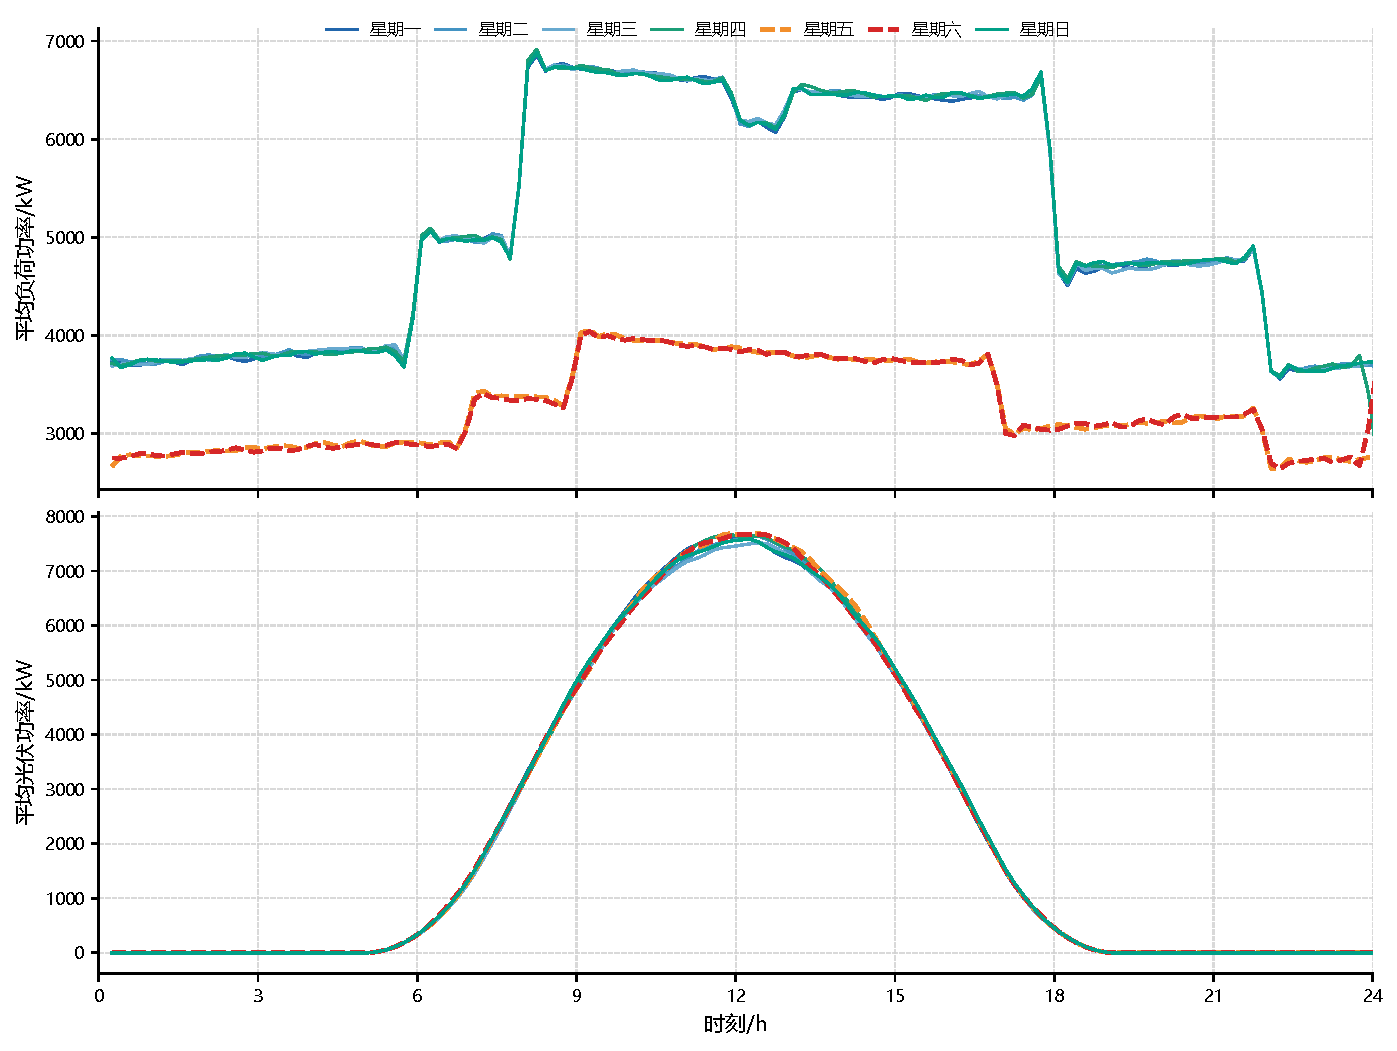
\includegraphics[width=0.72\textwidth]{../figures/问题二/问题二_星期一至星期日平均负荷与光伏曲线.pdf}
  \caption{星期一至星期日的平均负荷与光伏曲线}
  \label{fig:q2_weekday}
\end{figure}

为进一步确认周期结构，对每一天的 144 个时段取日均值，再基于全年 365 个日均值计算日尺度自相关函数，结果如图~\ref{fig:q2_acf} 所示。日均负荷在滞后 1 天、7 天与 14 天的自相关系数分别为 0.3732、0.9710 与 0.9424，后两者显著高于其余滞后，支持采用 7 天负荷周期；日均光伏对应为 0.9562、0.8780 与 0.7684，滞后 1 天即具有很高的相关性，支持采用日周期信息预测光伏。

\begin{figure}[H]
  \centering
  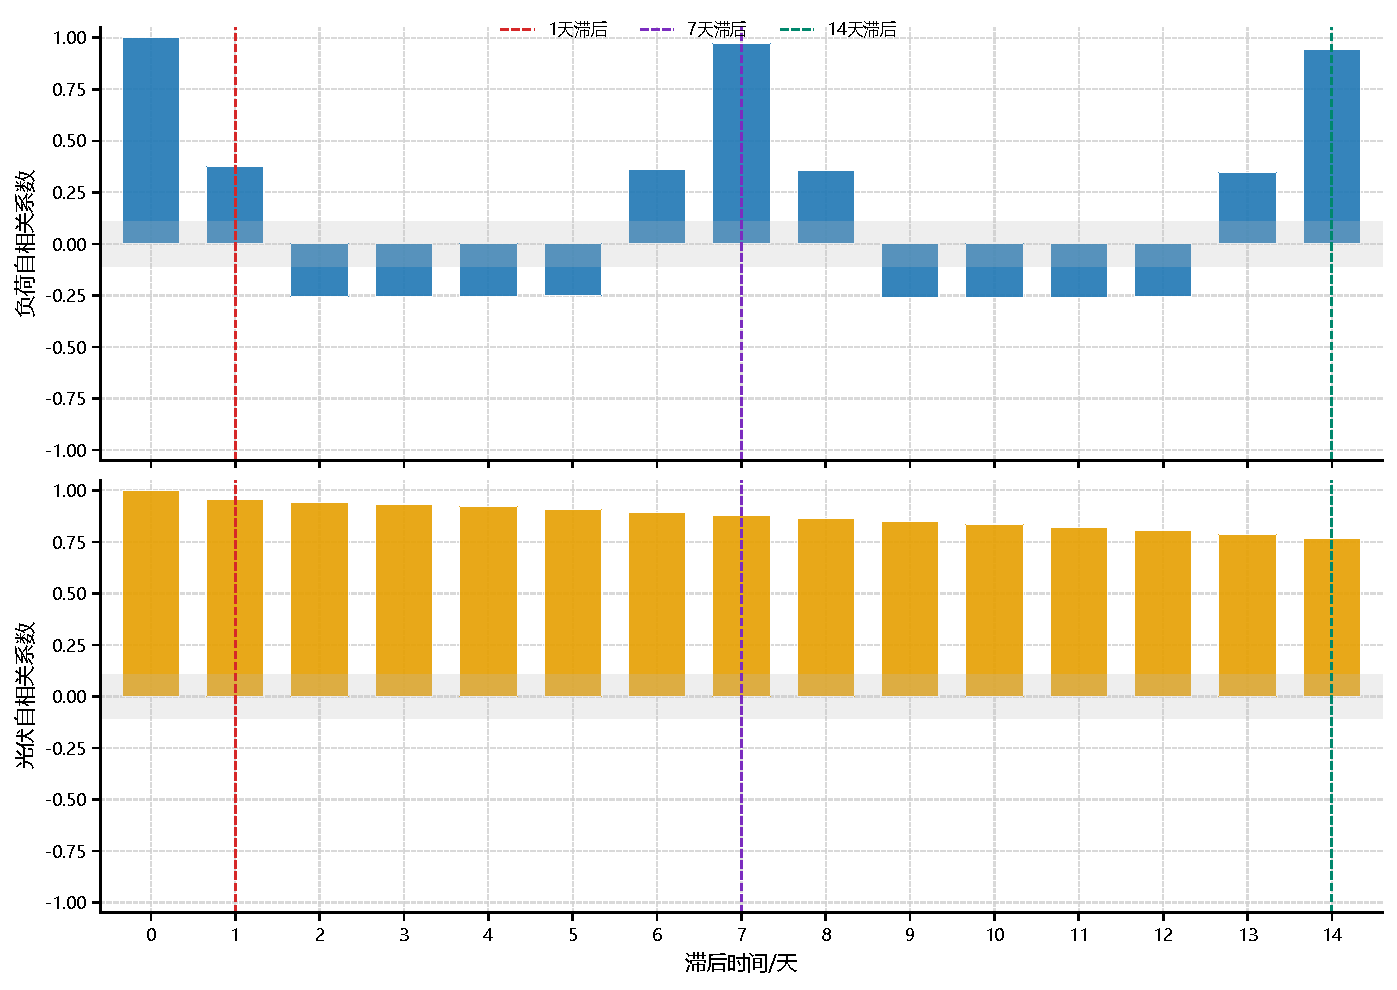
\includegraphics[width=0.72\textwidth]{../figures/问题二/问题二_负荷与光伏ACF.pdf}
  \caption{日均负荷与日均光伏的自相关函数}
  \label{fig:q2_acf}
\end{figure}

\subsubsection{预测精度}

对任一实际序列 $y_i$ 及其预测值 $\widehat y_i$，加权平均绝对百分比误差（WAPE）定义为

\begin{equation}
  \operatorname{WAPE}=\frac{\displaystyle\sum_{i=1}^{n}\left|y_i-\widehat y_i\right|}{\displaystyle\sum_{i=1}^{n}\left|y_i\right|}\times100\%.
  \label{eq:wape}
\end{equation}

式中：$i$ 为时段索引，$n$ 为评价时段数，$y_i$ 与 $\widehat y_i$ 分别为实际值和预测值；本研究中各评价量非负，故分母为评价期实际量总和。

在 2025 年 2 月 1 日至 12 月 31 日共 334 天、48096 个 10 分钟时段上，逐日向前预测的结果为：负荷平均绝对误差 29.902 kWh、均方根误差 41.701 kWh、WAPE 3.89\%；光伏全时段平均绝对误差 24.970 kWh、均方根误差 50.047 kWh、WAPE 6.30\%，非零时段平均绝对误差 44.669 kWh。所有误差均来自严格按时间向前的样本外预测，而非全年拟合后的样本内结果；指定日对比如图~\ref{fig:q2_day} 所示。

\begin{figure}[H]
  \centering
  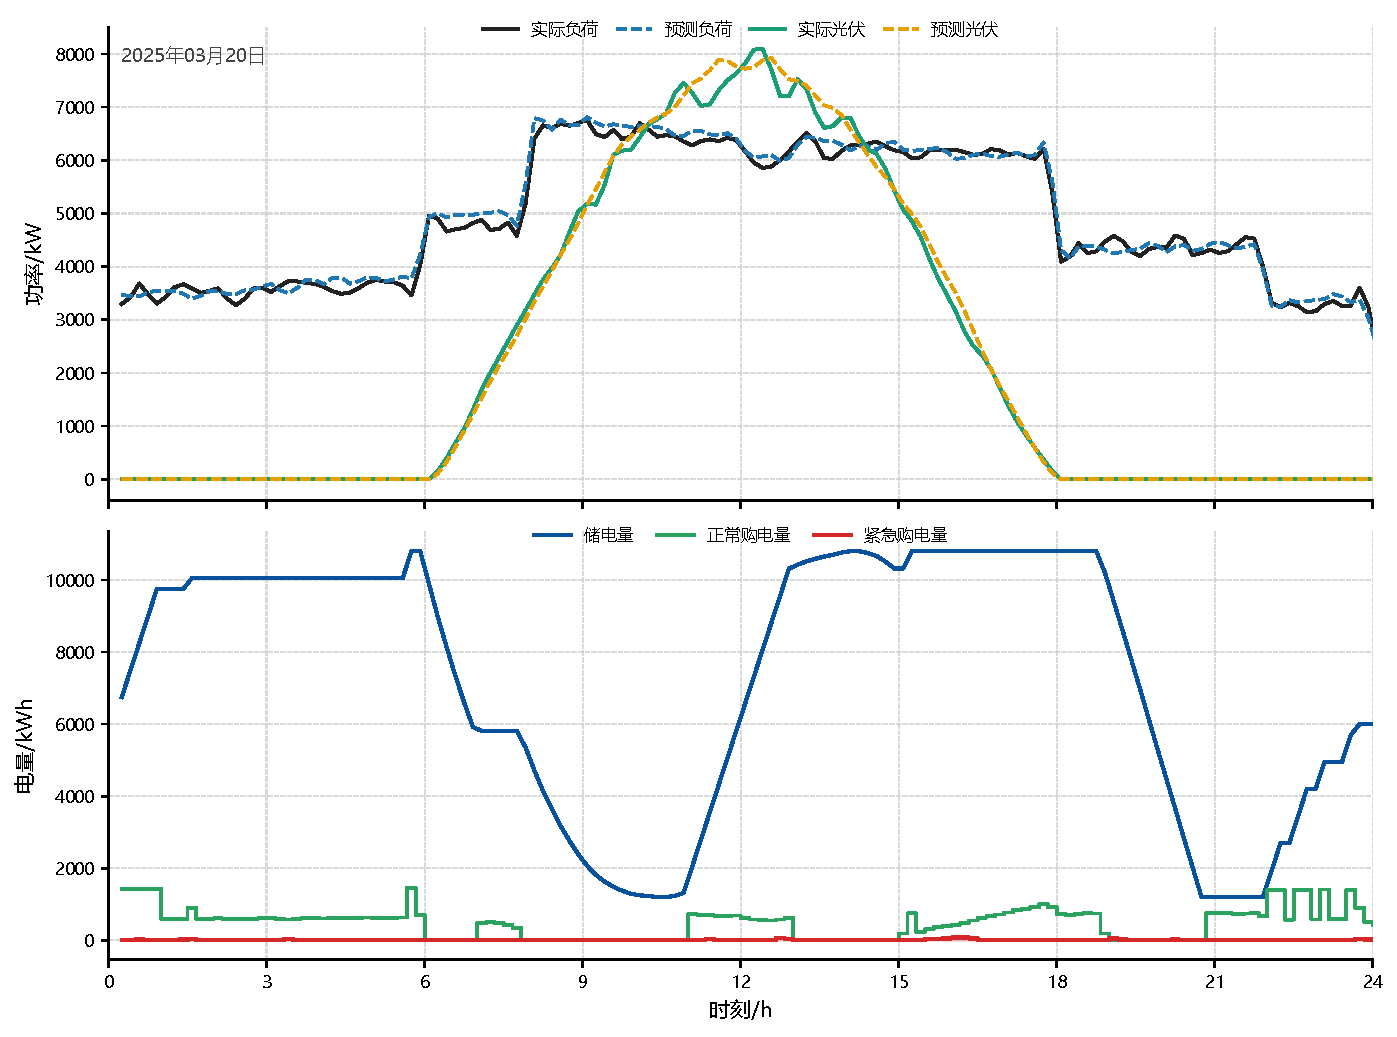
\includegraphics[width=0.72\textwidth]{../figures/问题二/问题二_24小时预测值与实际值.pdf}
  \caption{2025 年 3 月 20 日 24 小时预测值与实际值}
  \label{fig:q2_day}
\end{figure}

图~\ref{fig:q2_month} 给出 3 月日总电量的预测与实际对比，负荷的星期周期与光伏的缓慢季节变化均得到体现。

\begin{figure}[H]
  \centering
  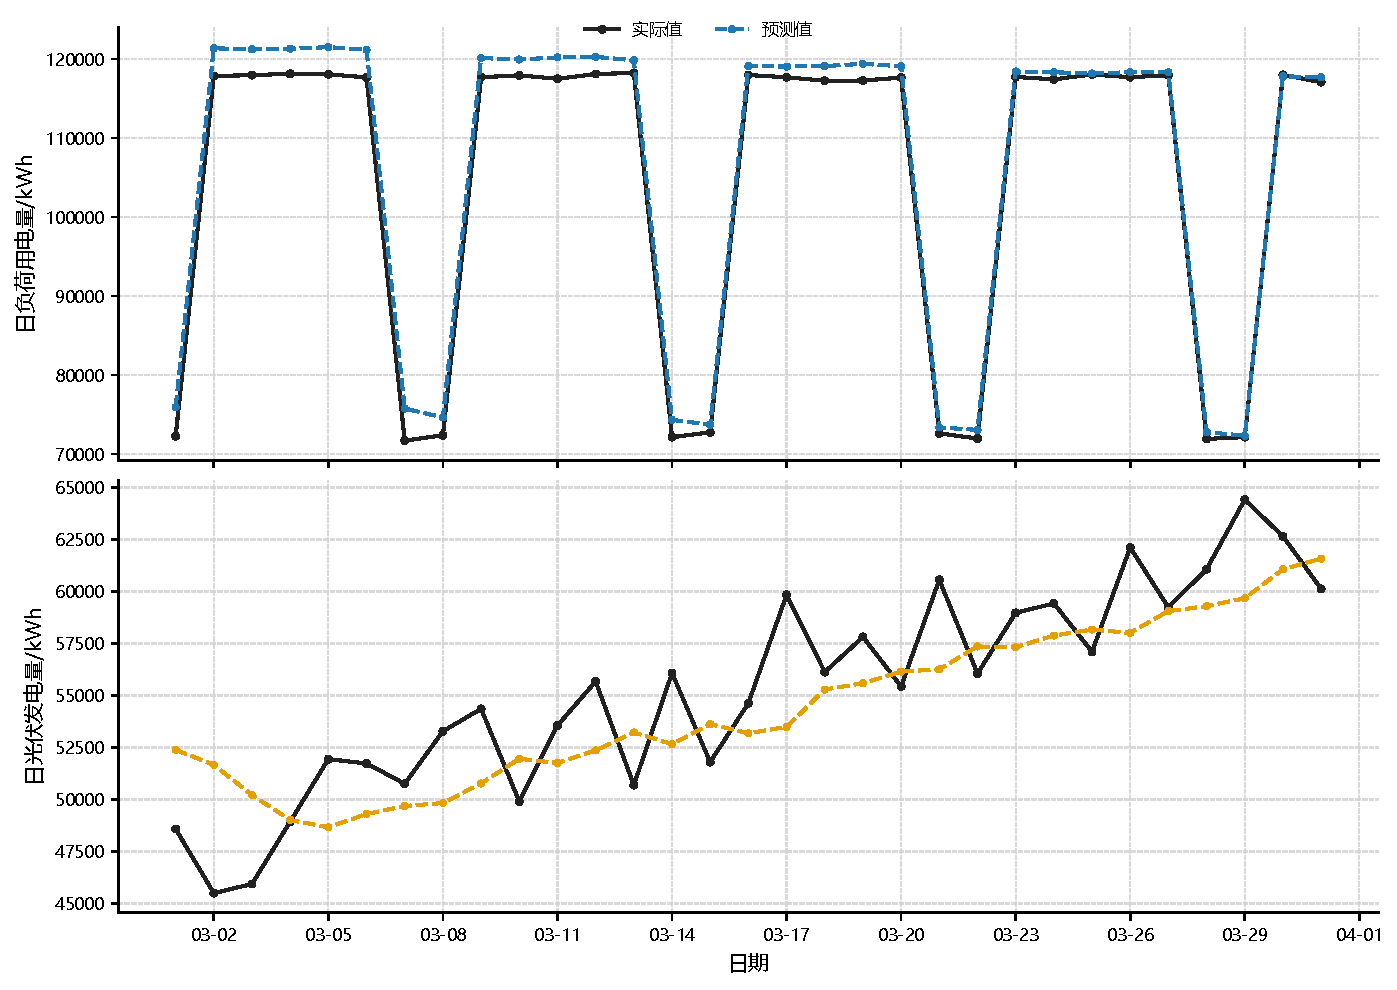
\includegraphics[width=0.72\textwidth]{../figures/问题二/问题二_一个月预测值与实际值.pdf}
  \caption{2025 年 3 月日总电量的预测值与实际值}
  \label{fig:q2_month}
\end{figure}

题目指定日期的完整购电、储能和紧急购电结果见表 6 至表 8。其中，12 月 21 日的计划购电量与购电费用最高，与冬季负荷较高、光伏出力较低的特征一致；储能设备在四个日期均呈现``夜间与午间低价时段充电、早晚高价时段放电''的套利特征。

\subsubsection{全年优化结果}

2025 年 2 月 1 日至 12 月 31 日共 334 天的全年汇总结果如表 5 所示。

{\footnotesize
\threelinetable{表 5\quad 问题二正式期全年汇总结果}{l r l r}{%
  \textbf{指标} & \textbf{结果} & \textbf{指标} & \textbf{结果}%
}{%
  正式天数 & 334 & 紧急购电费/元 & 1170588.48 \\
  计划购电量/kWh & 22069571.55 & 实际总费用/元 & 14637169.37 \\
  实际紧急购电量/kWh & 314788.59 & 平均日末储电量/kWh & 5993.78 \\
  实际富余电量/kWh & 3106105.93 & 日末储电量标准差/kWh & 541.93 \\
  正常购电费/元 & 13466580.90 & 12 月 31 日末储电量/kWh & 6626.15 \\
}
}

全年实际紧急购电量为 314788.59 kWh，约占计划购电量的 1.43\%；紧急购电费为 1170588.48 元，约占实际总费用的 8.00\%。平均日末储电量为 5993.78 kWh，标准差 541.93 kWh，说明日末储电量在季节基准与风险微调的共同作用下围绕软区间下沿小幅波动，而非固定在某一常数。全年逐日的正常购电量、紧急购电量与日末储电量如图~\ref{fig:q2_year} 所示。

\begin{figure}[H]
  \centering
  
\includegraphics[width=0.72\textwidth]{../figures/问题二/问题二_全年正常购电紧急购电与储电量.pdf}
  \caption{全年正常购电量、紧急购电量与日末储电量}
  \label{fig:q2_year}
\end{figure}

\subsubsection{指定日期的完整结果}

指定日期的购电、储能与紧急购电结果分别见表 6 至表 8。

{\scriptsize
\threelinetable{表 6\quad 问题二指定日期的购电结果}{l r r r r}{%
  \textbf{时间段} & \textbf{3 月 20 日} & \textbf{6 月 21 日} & \textbf{9 月 23 日} & \textbf{12 月 21 日}%
}{%
  10:00--10:10 & 0.00 & 0.00 & 0.00 & 0.00 \\
12:00--12:10 & 577.07 & 0.00 & 517.78 & 978.76 \\
14:00--14:10 & 0.00 & 0.00 & 0.00 & 0.00 \\
16:00--16:10 & 483.38 & 200.02 & 559.60 & 859.59 \\
18:00--18:10 & 700.06 & 0.00 & 825.99 & 727.46 \\
20:00--20:10 & 0.00 & 0.00 & 23.26 & 0.00 \\
全天购电量/kWh & 69205.65 & 37039.50 & 73127.51 & 97759.82 \\
全天购电费/元 & 45090.68 & 21942.35 & 47574.23 & 65454.20 \\
}

}

{\tiny
\begin{center}
  {\fontsize{10.5pt}{12.6pt}\heiti\bfseries 表 7\quad 问题二指定日期的储能结果}\par
  \vspace{0.25em}
  \resizebox{\textwidth}{!}{%
  \begin{tabular}{l r r r r r r r r}
    \toprule
    & \multicolumn{2}{c}{\textbf{3 月 20 日}} & \multicolumn{2}{c}{\textbf{6 月 21 日}} & \multicolumn{2}{c}{\textbf{9 月 23 日}} & \multicolumn{2}{c}{\textbf{12 月 21 日}} \\
    \cmidrule(lr){2-3}\cmidrule(lr){4-5}\cmidrule(lr){6-7}\cmidrule(lr){8-9}
    \textbf{时间段} & \textbf{充电量/kWh} & \textbf{放电量/kWh} & \textbf{充电量/kWh} & \textbf{放电量/kWh} & \textbf{充电量/kWh} & \textbf{放电量/kWh} & \textbf{充电量/kWh} & \textbf{放电量/kWh} \\
    \midrule
    0:00-4:00 & 3994.16 & 0.00 & 0.00 & 0.00 & 4701.99 & 0.00 & 3748.89 & 0.00 \\
4:00-8:00 & 833.33 & 5476.96 & 40.51 & 3473.19 & 833.33 & 5589.10 & 1666.67 & 1508.33 \\
8:00-12:00 & 5959.76 & 3163.04 & 6212.03 & 0.00 & 6188.17 & 3050.90 & 5833.33 & 7806.67 \\
12:00-16:00 & 5240.40 & 432.13 & 3794.87 & 0.00 & 4883.90 & 328.38 & 8177.36 & 2708.67 \\
16:00-20:00 & 0.00 & 5683.04 & 0.00 & 5971.81 & 0.00 & 5833.33 & 0.00 & 5620.93 \\
20:00-24:00 & 5806.94 & 2956.96 & 4697.87 & 2668.19 & 4980.19 & 2806.67 & 6478.83 & 3019.07 \\
0:00 储电量/kWh & \multicolumn{2}{c}{6455.25} & \multicolumn{2}{c}{5616.43} & \multicolumn{2}{c}{5818.21} & \multicolumn{2}{c}{6676.00} \\
24:00 储电量/kWh & \multicolumn{2}{c}{6426.24} & \multicolumn{2}{c}{5428.08} & \multicolumn{2}{c}{5682.17} & \multicolumn{2}{c}{7030.95} \\
    \bottomrule
  \end{tabular}%
  }
\end{center}
}

{\scriptsize
\threelinetable{表 8\quad 问题二指定日期的紧急购电结果}{l r l r l r l r}{%
  \textbf{3 月 20 日 时段} & \textbf{购电量/kWh} & \textbf{6 月 21 日 时段} & \textbf{购电量/kWh} & \textbf{9 月 23 日 时段} & \textbf{购电量/kWh} & \textbf{12 月 21 日 时段} & \textbf{购电量/kWh}%
}{%
  0:30-0:40 & 23.88 & 0:30-0:40 & 37.44 & 5:10-5:20 & 11.27 & 1:10-1:30 & 18.00 \\
1:10-1:50 & 57.91 & 1:30-1:40 & 40.00 & 5:50-6:00 & 1.20 & 1:40-2:00 & 18.50 \\
2:40-2:50 & 5.46 & 2:00-2:20 & 16.74 & 6:20-6:30 & 0.94 & 2:20-2:30 & 12.93 \\
3:10-3:40 & 73.60 & 3:00-3:40 & 62.95 & 7:00-7:10 & 5.93 & 3:10-3:30 & 54.51 \\
5:10-5:20 & 6.05 & 6:10-6:20 & 15.64 & 9:50-10:20 & 49.27 & 3:40-4:10 & 106.83 \\
10:00-10:10 & 4.85 & 19:10-19:20 & 21.22 & 11:00-11:10 & 42.26 & 4:20-4:30 & 0.23 \\
11:10-11:30 & 42.83 & 20:30-20:40 & 6.87 & 14:40-15:30 & 214.72 & 5:50-6:40 & 87.72 \\
12:40-13:00 & 90.14 &  &  & 16:00-16:20 & 58.72 & 10:30-11:50 & 451.32 \\
15:20-17:20 & 382.19 &  &  & 16:40-17:00 & 9.59 & 13:00-13:20 & 20.00 \\
18:20-18:30 & 2.55 &  &  & 20:30-20:40 & 10.11 & 17:30-17:40 & 7.98 \\
18:50-19:20 & 88.21 &  &  & 21:00-21:10 & 40.94 & 18:30-18:40 & 2.68 \\
20:00-20:30 & 24.35 &  &  & 22:30-22:40 & 6.00 & 18:50-19:10 & 4.07 \\
21:30-21:50 & 19.43 &  &  &  &  & 19:50-20:10 & 52.37 \\
23:40-0:00+1 & 55.73 &  &  &  &  & 23:00-23:10 & 9.65 \\
 &  &  &  &  &  & 23:40-23:50 & 0.61 \\
}
}


\subsubsection{终端储电量机制的对照分析}

在同一预测、随机种子和联合残差场景下，对四种终端处理方式进行对照。无终端约束、固定 6000 kWh 基准、季节余弦基准及季节基准叠加因果微调的全年费用依次为 14651641.38、14640006.24、14637301.67 和 14637169.37 元；对应的逐步节省额为 11635.14、2704.57 和 132.30 元。季节基准的贡献明显大于风险微调，说明终端机制主要避免跨日储能透支。

风险微调在正式期上调 189 天、下调 145 天，16 天触及 $+600$ kWh 截断上限，调整均值为 67.15 kWh。334 天的日末储电量均贴近当日软区间下沿，范围为 5105.04$\sim$7196.85 kWh，表明其作用是因果移动季节性最低备用曲线。四种方案的费用与储电量对比如图~\ref{fig:q2_reserve} 所示。

\begin{figure}[H]
  \centering
  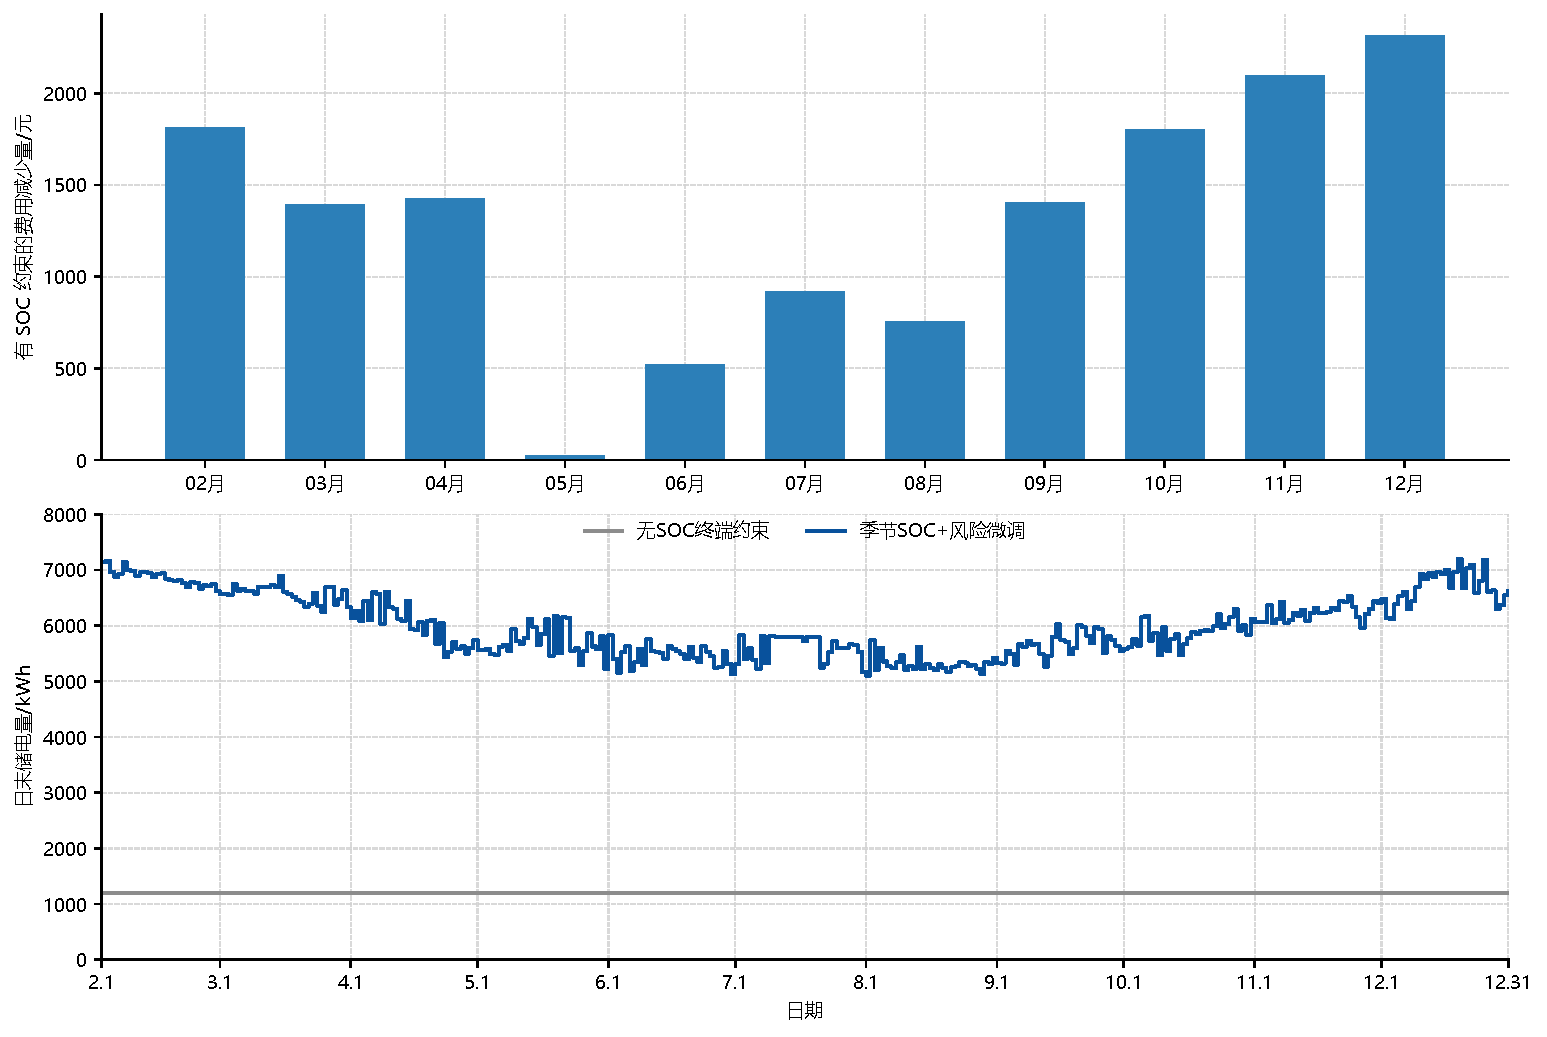
\includegraphics[width=0.72\textwidth]{../figures/问题二/问题二_日备不足惩罚前后费用与储能对比.pdf}
  \caption{有、无终端储电量约束方案的费用与日末储电量对比}
  \label{fig:q2_reserve}
\end{figure}
